% BDE Guide --- Chapter 5: University Core (ICC + CSL)
\chapter{University Core: ICC \& Career Skills}
\label{ch:university-core}

\begin{quote}
\emph{``NTU wants every graduate --- engineer or historian --- to be digitally literate, ethically grounded, and career-ready.''} University Core is that common contract. It is not BDE, not College Core, and not optional.
\end{quote}

\noindent\fbox{\parbox{\dimexpr\linewidth-2\fboxsep-2\fboxrule}{%
\textbf{From zero: University Core defined.} University Core $=$ the \emph{NTU-wide} compulsory spine for every undergraduate (all colleges, all programmes). It comprises the Interdisciplinary Collaborative Core (ICC, CC0001--CC0007) plus Career \& Innovative Enterprise for the Future World (ML0004, CSL). Total: 17~AU. We cover each course's purpose, AU, and how ICC differs from BDE/College Core.}}
\vspace{0.4em}

\section*{Learning Outcomes}
After this chapter you will be able to:
\begin{enumerate}[label=(L\arabic*)]
    \item list every University Core component (CC0001--CC0007 + ML0004), AU, and typical year;
    \item explain the ICC's five learning pillars and why CS students take ICC alongside computing cores;
    \item distinguish University Core from College Core and BDE (no double-counting);
    \item describe ML0004 (CSL) and its career-preparation purpose;
    \item locate ICC/CSL in your timetable and Degree Audit.
\end{enumerate}

% ============================================================
\section{What Is University Core?}
\label{sec:what-icc}

\begin{definition}[University Core (ICC + CSL) --- 17~AU]
University Core is NTU-wide: every undergraduate, from CCDS to HSS to Business, takes the same spine (with minor college-specific variants in delivery). It has two parts:
\begin{itemize}
    \item \textbf{Interdisciplinary Collaborative Core (ICC)} --- CC0001, CC0002, CC0003, CC0005, CC0006, CC0007 (15~AU combined).
    \item \textbf{Career \& Innovative Enterprise for the Future World (CSL)} --- ML0004 (2~AU).
\end{itemize}
Total: 17~AU. University Core is \emph{not} BDE and \emph{not} College Core; a course counted as ICC cannot also count as BDE. Table~\ref{tab:au-buckets} in the Appendix shows the full 135~AU map.
\end{definition}

\begin{figure}[h]
\centering
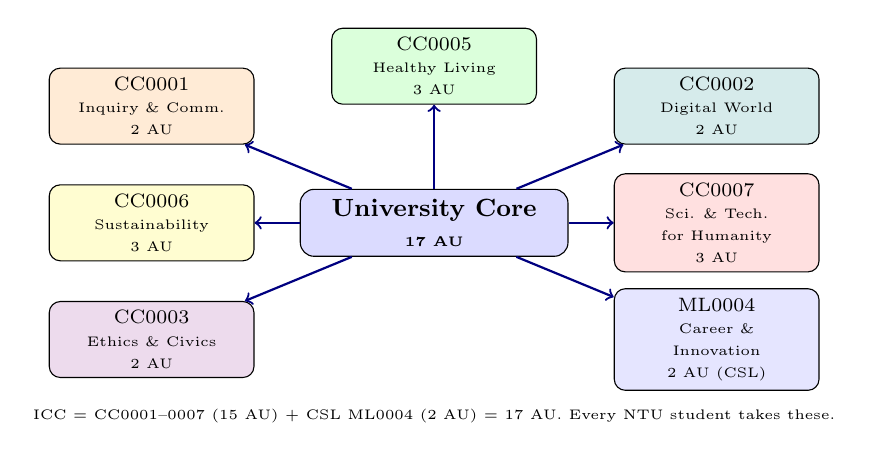
\begin{tikzpicture}[scale=0.78,every node/.style={font=\scriptsize}]
% ICC hexagon / flower with centre
\node[draw,fill=blue!14,rounded corners=5pt,minimum width=3.4cm,minimum height=0.85cm,align=center,font=\small\bfseries] (centre) at (0,0) {University Core\\{\tiny 17 AU}};
% ICC nodes around
\node[draw,fill=orange!16,rounded corners=4pt,minimum width=2.6cm,minimum height=0.75cm,align=center] (cc1) at (-4.6,1.9) {CC0001\\{\tiny Inquiry \& Comm.}\\{\tiny 2 AU}};
\node[draw,fill=teal!16,rounded corners=4pt,minimum width=2.6cm,minimum height=0.75cm,align=center] (cc2) at (4.6,1.9) {CC0002\\{\tiny Digital World}\\{\tiny 2 AU}};
\node[draw,fill=violet!14,rounded corners=4pt,minimum width=2.6cm,minimum height=0.75cm,align=center] (cc3) at (-4.6,-1.9) {CC0003\\{\tiny Ethics \& Civics}\\{\tiny 2 AU}};
\node[draw,fill=green!14,rounded corners=4pt,minimum width=2.6cm,minimum height=0.75cm,align=center] (cc5) at (0,2.55) {CC0005\\{\tiny Healthy Living}\\{\tiny 3 AU}};
\node[draw,fill=yellow!18,rounded corners=4pt,minimum width=2.6cm,minimum height=0.75cm,align=center] (cc6) at (-4.6,0) {CC0006\\{\tiny Sustainability}\\{\tiny 3 AU}};
\node[draw,fill=red!12,rounded corners=4pt,minimum width=2.6cm,minimum height=0.75cm,align=center] (cc7) at (4.6,0) {CC0007\\{\tiny Sci. \& Tech.}\\{\tiny for Humanity}\\{\tiny 3 AU}};
\node[draw,fill=blue!10,rounded corners=4pt,minimum width=2.6cm,minimum height=0.75cm,align=center] (ml) at (4.6,-1.9) {ML0004\\{\tiny Career \&}\\{\tiny Innovation}\\{\tiny 2 AU (CSL)}};
\foreach \target in {cc1,cc2,cc3,cc5,cc6,cc7,ml} \draw[->,thick,blue!50!black] (centre) -- (\target);
\node[font=\tiny,align=center,fill=white,inner sep=2pt] at (0,-3.15) {ICC $=$ CC0001--0007 (15 AU) + CSL ML0004 (2 AU) $=$ 17 AU. Every NTU student takes these.};
\end{tikzpicture}
\caption{University Core flower: every petal is compulsory. No ICC course can be double-counted as BDE.}
\label{fig:icc-flower}
\end{figure}

% ============================================================
\section{The ICC Courses in Detail}
\label{sec:icc-courses}

\subsection{CC0001 Inquiry \& Communication in an Interdisciplinary World (2~AU)}
\paragraph{Purpose.} Academic inquiry, critical reading, argument construction, and written/oral communication across disciplines. You learn to ask good questions, evaluate evidence, and present an argument --- not just to write essays.

\paragraph{When.} Y1 S1 for most CCDS cohorts. Prerequisite for HW0288 (College Core) and for CC0003 in some pathways.

\paragraph{Why CS students need it.} Design docs, RFCs, incident reports, and paper reviews all require inquiry + communication. CC0001 is the foundation; HW0288 later specialises it for engineering contexts.

\subsection{CC0002 Navigating the Digital World (2~AU)}
\paragraph{Purpose.} Digital literacy for every NTU graduate: data, AI, cybersecurity, and digital ethics at a conceptual level --- not coding, but understanding the digital society you will build systems for.

\paragraph{For CS students.} Much of CC0002 will feel familiar (you go deeper in SC1005/SC2006/SC3010). Treat it as the ``explain it to a non-CS friend'' version --- valuable precisely because you will need to explain CS to non-CS stakeholders.

\subsection{CC0003 Ethics \& Civics in a Multicultural World (2~AU)}
\paragraph{Purpose.} Ethical reasoning, civic responsibility, and multicultural competence in Singapore and globally. Case studies on technology ethics, inequality, and governance.

\paragraph{For CS students.} Directly relevant to AI ethics, algorithmic bias, data privacy (PDPA/GDPR), and responsible deployment --- themes that recur in SC3000, SC3010, and your future professional practice.

\subsection{CC0005 Healthy Living \& Wellbeing (3~AU)}
\paragraph{Purpose.} Physical health, mental wellbeing, and resilience. Includes pathways HW0001/HW0002 for students who need bridging.

\paragraph{Format.} Often blended --- lectures + activity-based components (fitness, mindfulness, health literacy). Assessment is typically quizzes + reflection + participation rather than a heavy exam.

\subsection{CC0006 Sustainability: Society, Economy \& Environment (3~AU)}
\paragraph{Purpose.} Climate, sustainability, circular economy, and the UN Sustainable Development Goals. Interdisciplinary by design --- you collaborate with students from other colleges.

\paragraph{For CS students.} Sustainable computing (energy-efficient systems, green AI, e-waste) connects directly. Several MPE and BDE sustainability modules (ES9001, CM8001) deepen this --- but CC0006 itself is University Core, not BDE.

\subsection{CC0007 Science \& Technology for Humanity (3~AU)}
\paragraph{Purpose.} How science and technology shape humanity --- history of technology, innovation, science communication, and societal impact.

\paragraph{For CS students.} The ``why should society trust your system?'' course. Useful framing for FYP/Capstone impact sections and for communicating technical work to non-technical audiences.

% ============================================================
\section{ML0004 Career \& Innovative Enterprise for the Future World (2~AU, CSL)}
\label{sec:ml0004}

\begin{definition}[CSL: Career Skills \& Language? No --- Career \& Innovative Enterprise]
ML0004 is the \emph{Career \& Innovative Enterprise for the Future World} module (2~AU), classified as Career Skills \& Leadership (CSL) in some summaries. It is distinct from the Centre for Modern Languages (also ``language'' in other contexts) --- same acronym space, different meaning. In University Core counting, ML0004 is the CSL component that brings University Core from 15~AU (ICC alone) to 17~AU.
\end{definition}

\paragraph{Purpose.} Career readiness: self-awareness, industry exploration, r\'esum\'e and interview skills, networking, innovation and enterprise mindset. Delivered as workshops, industry talks, and reflective assignments rather than lectures + exam.

\paragraph{When.} Typically Y2--Y3; some cohorts take it in Y1 S2. Check your study plan --- timing shifts by cohort.

\paragraph{Why it matters.} It is the only compulsory course explicitly about \emph{getting and succeeding in} the internship (SC3920) and first job. Skipping its r\'esum\'e/interview preparation before Y3 S2 internship applications is a common regret.

\begin{figure}[h]
\centering
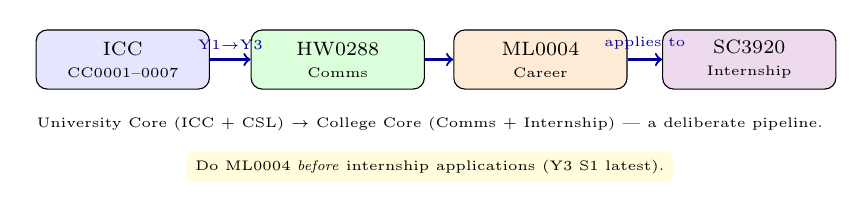
\begin{tikzpicture}[scale=0.78,every node/.style={font=\scriptsize}]
% Pipeline from ICC to career
\node[draw,fill=blue!10,rounded corners=4pt,minimum width=2.2cm,minimum height=0.75cm,align=center] (a) at (-5.0,0) {ICC\\{\tiny CC0001--0007}};
\node[draw,fill=green!14,rounded corners=4pt,minimum width=2.2cm,minimum height=0.75cm,align=center] (b) at (-1.5,0) {HW0288\\{\tiny Comms}};
\node[draw,fill=orange!16,rounded corners=4pt,minimum width=2.2cm,minimum height=0.75cm,align=center] (c) at (1.8,0) {ML0004\\{\tiny Career}};
\node[draw,fill=violet!14,rounded corners=4pt,minimum width=2.2cm,minimum height=0.75cm,align=center] (d) at (5.2,0) {SC3920\\{\tiny Internship}};
\draw[->,thick,blue!60!black] (a) -- (b) node[midway,above,font=\tiny] {Y1$\to$Y3};
\draw[->,thick,blue!60!black] (b) -- (c);
\draw[->,thick,blue!60!black] (c) -- (d) node[midway,above,font=\tiny] {applies to};
\node[font=\tiny,align=center] at (0,-1.05) {University Core (ICC + CSL) $\to$ College Core (Comms + Internship) --- a deliberate pipeline.};
\node[font=\tiny,align=center,fill=yellow!14,rounded corners=2pt,inner sep=3pt] at (0,-1.75) {Do ML0004 \emph{before} internship applications (Y3 S1 latest).};
\end{tikzpicture}
\caption{From University Core to workplace: ICC builds breadth, HW0288 hones engineering communication, ML0004 prepares the r\'esum\'e, SC3920 tests it in industry.}
\label{fig:icc-to-career}
\end{figure}

% ============================================================
\section{University Core vs.\ College Core vs.\ BDE}
\label{sec:core-vs-bde}

\begin{table}[h]
\centering
\small
\renewcommand{\arraystretch}{1.25}
\begin{tabular}{@{}p{2.8cm} c p{3.2cm} p{4.5cm}@{}}
\toprule
Bucket & AU & Owner & Can you choose? \\
\midrule
University Core (ICC+CSL) & 17 & NTU (all colleges) & No --- every course fixed \\
College Core & 16 & CCDS & No --- SC1003/HW0288/SC3920 fixed \\
Programme Core & 47 & CCDS-CS & No --- SC1004--SC3099 fixed \\
MPE & 35 & CCDS-CS & Semi --- choose 9 from SC3xxx/4xxx list \\
BDE & 20 & You & Yes --- any approved NTU course \\
\midrule
\multicolumn{4}{@{}p{\linewidth}@{}} {\footnotesize AU per curriculum-page bucketing; PDF F-Core bucketing shows College 15 + BDE 21 for same courses. Total 135 invariant; Degree Audit authoritative.} \\
\bottomrule
\end{tabular}
\end{table}

\begin{remark}[No double-counting across cores]
A course counted as University Core (e.g., CC0002) cannot also satisfy College Core or BDE, even if its content overlaps with a CS-adjacent BDE. Degree Audit enforces one-bucket-per-course. If you take an extra CC-coded course beyond the required ICC, the \emph{extra} one may count as BDE --- but the required ICC ones never do.
\end{remark}

% ============================================================
\section{Chapter Notes}
University Core structure per NTU Interdisciplinary Collaborative Core (ICC) programme pages and NTU Academic Regulations (AY2024--25). Course purposes summarised from NTU Course Catalogue entries for CC0001--CC0007 and ML0004 at time of writing; titles and AUs confirmed against CCDS BSc (Hons) in Computer Science study plan PDF. Offerings and delivery mode vary by semester and cohort; Degree Audit is authoritative.

% ============================================================
\section{Exercises}
\label{sec:ch05-exercises}
\begin{enumerate}[label=E5.\arabic*, leftmargin=*, itemsep=0.8em]
    \item \textbf{AU check.} List the AU for each University Core course and verify the total is 17. Which component is CSL, and how many AU does it carry?
    \item \textbf{Bucket confusion.} A friend says ``I will count CC0002 as a BDE because it is about digital literacy and I am a CS student''. Why is this incorrect?
    \item \textbf{Career pipeline.} Arrange CC0001, HW0288, ML0004, and SC3920 in the order you should take them, and explain the dependency.
    \item \textbf{Degree Audit.} After Y1, Degree Audit shows CC0005 as ``Outstanding'' though you passed a sustainability BDE (ES9001). Why does ES9001 not satisfy CC0006, and what must you do?
\end{enumerate}
% End of Chapter 5
